% ============================================================
%  Chapter: Optimization Action Analyzer
%  Part of the graduation project documentation
%
%  Required preamble packages (add to your main document if not
%  already present):
%    \usepackage{graphicx}
%    \usepackage{listings}
%    \usepackage{xcolor}
%    \usepackage{booktabs}
%    \usepackage{longtable}
%    \usepackage{hyperref}
%    \usepackage{tikz}
%    \usetikzlibrary{arrows.meta, positioning, shapes.geometric}
%    \usepackage{caption}
%    \usepackage{amsmath}
% ============================================================

\chapter{Optimization Action Analyzer}
\label{chap:opt-action-analyzer}

\section{Introduction}
Radio Access Network (RAN) optimization teams routinely push configuration
changes to live network elements --- antenna tilt adjustments, transmit
power tuning, handover parameter updates, carrier-aggregation activation,
and similar tuning actions. A recurring, largely manual problem faced by
these teams is answering a simple but operationally critical question:

\begin{quote}
\emph{``Did the change we just made actually improve the network, and by
how much?''}
\end{quote}

Answering this question correctly requires (i) knowing precisely
\textbf{what} changed and \textbf{when}, (ii) selecting a fair
\textbf{baseline} period against which to compare performance, and
(iii) quantifying the impact across dozens of Key Performance Indicators
(KPIs) while accounting for the strong diurnal and weekly seasonality that
characterises telecom traffic.

The \textbf{Optimization Action Analyzer} (internally named the
\emph{NetOps Impact Analyzer}) is a web-based analytical tool built to
automate this workflow end-to-end. It couples a version-controlled
database of network configuration changes with a KPI time-series
warehouse, and produces an interactive before/after impact analysis for
any configuration change --- without requiring the analyst to manually
export data, align time windows, or build charts in a spreadsheet.

\section{Motivation and Problem Statement}
Traditional post-optimization impact analysis in telecom operations
suffers from several recurring issues:

\begin{itemize}
    \item \textbf{No single source of truth for ``what changed''.}
        Configuration changes are often tracked informally (tickets,
        spreadsheets, chat messages), making it difficult to reconstruct
        an accurate timeline of network actions.
    \item \textbf{Naive before/after comparisons are biased.}
        Comparing a Monday after a change to the previous day (Sunday)
        ignores weekly traffic seasonality and produces misleading
        conclusions.
    \item \textbf{Overlapping changes confound results.}
        If a second optimization action occurs shortly after the first,
        naive analysis windows will blend the effects of both changes.
    \item \textbf{Manual, non-repeatable analysis.}
        Without tooling, every impact assessment is a bespoke, one-off
        spreadsheet exercise that is slow and error-prone.
\end{itemize}

The Optimization Action Analyzer directly addresses each of these issues
by combining a \textbf{version-controlled configuration database (Dolt)}
with a \textbf{weekday-matched statistical comparison engine} and an
\textbf{interactive visualization layer}.

\section{System Architecture}
The application follows a clean layered architecture that separates data
access, data processing, visualization, configuration persistence, and UI
orchestration. This separation of concerns keeps each module independently
testable and allows the underlying database or charting library to be
replaced with minimal impact on the rest of the system.

\begin{figure}[htbp]
    \centering
    \begin{tikzpicture}[
        node distance=10mm and 16mm,
        box/.style={draw, rounded corners, minimum width=3.6cm,
                     minimum height=1.1cm, align=center, font=\small,
                     fill=blue!6},
        arrow/.style={-{Latex[length=2mm]}, thick}
    ]
        \node[box, fill=blue!15] (app) {\texttt{app.py}\\Streamlit UI Orchestration};
        \node[box, below left=of app] (db) {\texttt{db.py}\\Dolt / PyMySQL\\Data Access};
        \node[box, below=of app] (data) {\texttt{data.py}\\Pandas Wrangling\\Hunk \& Matching Logic};
        \node[box, below right=of app] (viz) {\texttt{viz.py}\\Plotly Chart\\Builders};
        \node[box, right=of app] (config) {\texttt{config.py}\\KPI Polarity\\Persistence (JSON)};
        \node[box, below=of db, fill=gray!10] (dolt) {Dolt SQL Server\\\texttt{network\_kpis},\\\texttt{dolt\_log}};

        \draw[arrow] (app) -- (db);
        \draw[arrow] (app) -- (data);
        \draw[arrow] (app) -- (viz);
        \draw[arrow] (app) -- (config);
        \draw[arrow] (db) -- (dolt);
        \draw[arrow] (db) -- (data);
        \draw[arrow] (data) -- (viz);
    \end{tikzpicture}
    \caption{High-level module architecture of the Optimization Action
    Analyzer. The Streamlit application (\texttt{app.py}) orchestrates
    calls into four independent layers: database access, data wrangling,
    visualization, and configuration persistence.}
    \label{fig:architecture}
\end{figure}

Table~\ref{tab:modules} summarises the responsibility of each module.

\begin{table}[htbp]
    \centering
    \caption{Module responsibilities}
    \label{tab:modules}
    \begin{tabular}{@{}p{2.4cm}p{9.5cm}@{}}
        \toprule
        \textbf{Module} & \textbf{Responsibility} \\
        \midrule
        \texttt{db.py}     & Establishes the connection to the Dolt SQL
                              server (or falls back to a synthetic mock
                              data generator for development/demo),
                              discovers KPI columns from the schema, and
                              exposes query functions for the commit log,
                              commit diffs, and KPI time-series. \\
        \texttt{data.py}   & Pure-pandas transformation layer: groups raw
                              commits into daily \emph{Action Hunks},
                              resolves the rolling evaluation window,
                              and builds weekday-matched Before/After
                              KPI profiles (aggregated and per-day). \\
        \texttt{viz.py}    & Builds all Plotly figures --- the action
                              timeline, the Before/After trend chart, the
                              interval delta bar chart --- and constructs
                              the tabular KPI impact summary. \\
        \texttt{config.py} & Persists the user-defined optimization
                              polarity (``higher is better'' vs. ``lower
                              is better'') for every KPI to
                              \texttt{kpi\_config.json}, inferring
                              sensible defaults from column-name
                              keywords on first run. \\
        \texttt{app.py}    & Streamlit front-end: wires the other four
                              modules together, renders the sidebar,
                              controls, charts, and summary table, and
                              manages Streamlit's caching layer. \\
        \bottomrule
    \end{tabular}
\end{table}

\section{Data Model and Sources}
The analyzer consumes two logical data sources, both served through a
\textbf{Dolt} SQL server (a version-controlled, Git-like relational
database) via \texttt{PyMySQL}:

\begin{enumerate}
    \item \textbf{\texttt{network\_kpis}} --- a time-series table of
        network performance counters at fixed granularity (15-minute
        intervals in the reference deployment), including metrics such
        as downlink/uplink throughput, drop rate, RACH success rate,
        CQI, BLER, latency, PRB utilization, handover success rate, and
        SINR.
    \item \textbf{\texttt{dolt\_log}} --- Dolt's built-in commit history
        system table, giving a full audit trail of every configuration
        change: commit hash, committer, e-mail, timestamp, and commit
        message. Because Dolt versions the configuration tables
        themselves (e.g. \texttt{cell\_config}, \texttt{rf\_config}),
        the per-commit \textbf{diff} (which columns changed, from what
        value to what value) can be retrieved directly through Dolt's
        \texttt{dolt\_diff\_<table>} system views.
\end{enumerate}

This design means the tool requires \emph{no separate change-management
system}: the database's own version history \emph{is} the action log,
guaranteeing that the recorded timeline of changes is always accurate and
tamper-evident.

For development and demonstration purposes, \texttt{db.py} includes a
\texttt{USE\_MOCK\_DATA} switch that generates realistic synthetic KPI
data (diurnal traffic patterns plus an injected post-action uplift) and a
fabricated five-hunk commit log, allowing the full pipeline to be
exercised without a live Dolt instance.

\section{Core Algorithms}

\subsection{Action Hunks: Grouping Commits by Calendar Day}
Individual commits are rarely meaningful in isolation --- an optimization
action typically spans several related configuration commits performed
within the same maintenance window. \texttt{build\_action\_hunks()} groups
all commits sharing the same calendar date into a single \emph{Action
Hunk}, producing, for each hunk, a human-readable label (e.g.
\texttt{"2024-06-10 (Mon) · 3 commits"}) and the list of underlying
commit records. This gives the analyst one clean, selectable unit of
change per optimization event rather than a noisy list of individual
commits.

\subsection{Rolling Evaluation Window}
Once a hunk is selected, \texttt{resolve\_eval\_window()} determines the
``After'' period over which impact will be measured:

\begin{itemize}
    \item The window always starts on the hunk's date.
    \item By default, the window ends either \emph{today} or the day
        before the \emph{next} recorded hunk --- whichever is earlier ---
        so that the effect of a later change is never mixed into the
        current analysis.
    \item An \textbf{``Ignore Next Action Hunk''} toggle lets the analyst
        override this cap and extend the window through to the present
        day when a later change is known to be unrelated or negligible.
\end{itemize}

\subsection{Weekday-Matched Baseline Construction}
Naively comparing the day after a change to the day before it is
statistically unsound because telecom traffic exhibits strong weekly
seasonality (weekday vs. weekend, business-hours peaks, etc.). The
analyzer instead uses \texttt{collect\_matching\_weekdays()}, which:

\begin{enumerate}
    \item For every date in the After window, computes the exact
        same weekday exactly \textbf{seven days earlier} as its
        matching Before date.
    \item Averages KPI values across all After-window dates sharing the
        same minute-of-day index (0--1439), and separately averages the
        corresponding Before dates.
    \item Aligns both resulting profiles to a common minute-of-day
        index so that Before and After curves are directly comparable.
\end{enumerate}

This produces statistically fair, seasonality-normalised Before/After
profiles even for multi-week evaluation windows. A companion function,
\texttt{collect\_individual\_days()}, preserves the same matching logic
without averaging, grouping every individual After day (and its matched
Before day) by weekday name, so an analyst can drill into a specific
day's behaviour rather than only viewing the aggregate.

\subsection{Optimization Polarity}
Not every KPI improves by increasing: a rise in throughput is good, while
a rise in drop rate or latency is bad. \texttt{config.py} maintains a
persistent \textbf{polarity map} (\texttt{"higher"} or \texttt{"lower"}
is better) for every discovered KPI. On first run, polarity is inferred
automatically from column-name keywords (e.g. \texttt{drop}, \texttt{error},
\texttt{latency}, \texttt{bler}, \texttt{retry} $\Rightarrow$ lower is
better); the analyst can override and persist any KPI's polarity from the
sidebar, and the choice is written to \texttt{kpi\_config.json} so it
survives application restarts. This polarity map drives the colour-coding
(improved / degraded) used throughout the delta chart and the summary
table.

\section{Visualization Layer}
All charts are built with Plotly and share a consistent dark,
telecom-operations-console visual theme (navy background, cyan/green/red
accent palette, monospace font) defined centrally in \texttt{viz.py}.

\begin{description}
    \item[Action Timeline] (\texttt{plot\_action\_timeline}) --- a
        horizontal HUD-style timeline where each marker represents one
        Action Hunk; marker size and colour encode the number of commits,
        and hovering reveals full commit metadata (hash, committer,
        e-mail, timestamp, message) for every commit in that hunk.

    \item[KPI Trend --- Aggregated Mode] (\texttt{plot\_kpi\_trend}) --- a
        dual-line overlay of the averaged Before and After minute-of-day
        profiles for the selected KPI, with optional vertical markers
        annotating the exact commit timestamps inside the evaluation
        window.

    \item[KPI Trend --- Individual-Day Mode]
        (\texttt{plot\_kpi\_trend\_individual}) --- one figure per
        weekday, overlaying every individual After day against its
        matched Before day, with an optional bold mean-overlay trace per
        weekday group.

    \item[Interval Delta Bars] (\texttt{plot\_delta\_bars}) --- a
        polarity-aware bar chart of (After $-$ Before) at every
        minute-of-day interval, coloured green where the change is an
        improvement and red where it is a degradation, based on the
        KPI's configured polarity.

    \item[KPI Impact Summary Table] (\texttt{build\_summary\_table}) ---
        a single table covering \emph{every} discovered KPI in one view:
        Before average, After average, absolute change, percentage
        change, and a colour-coded Improved / Degraded / No-Change
        status, giving the analyst an at-a-glance verdict on the overall
        health impact of the optimization action.
\end{description}

\begin{figure}[htbp]
    \centering
    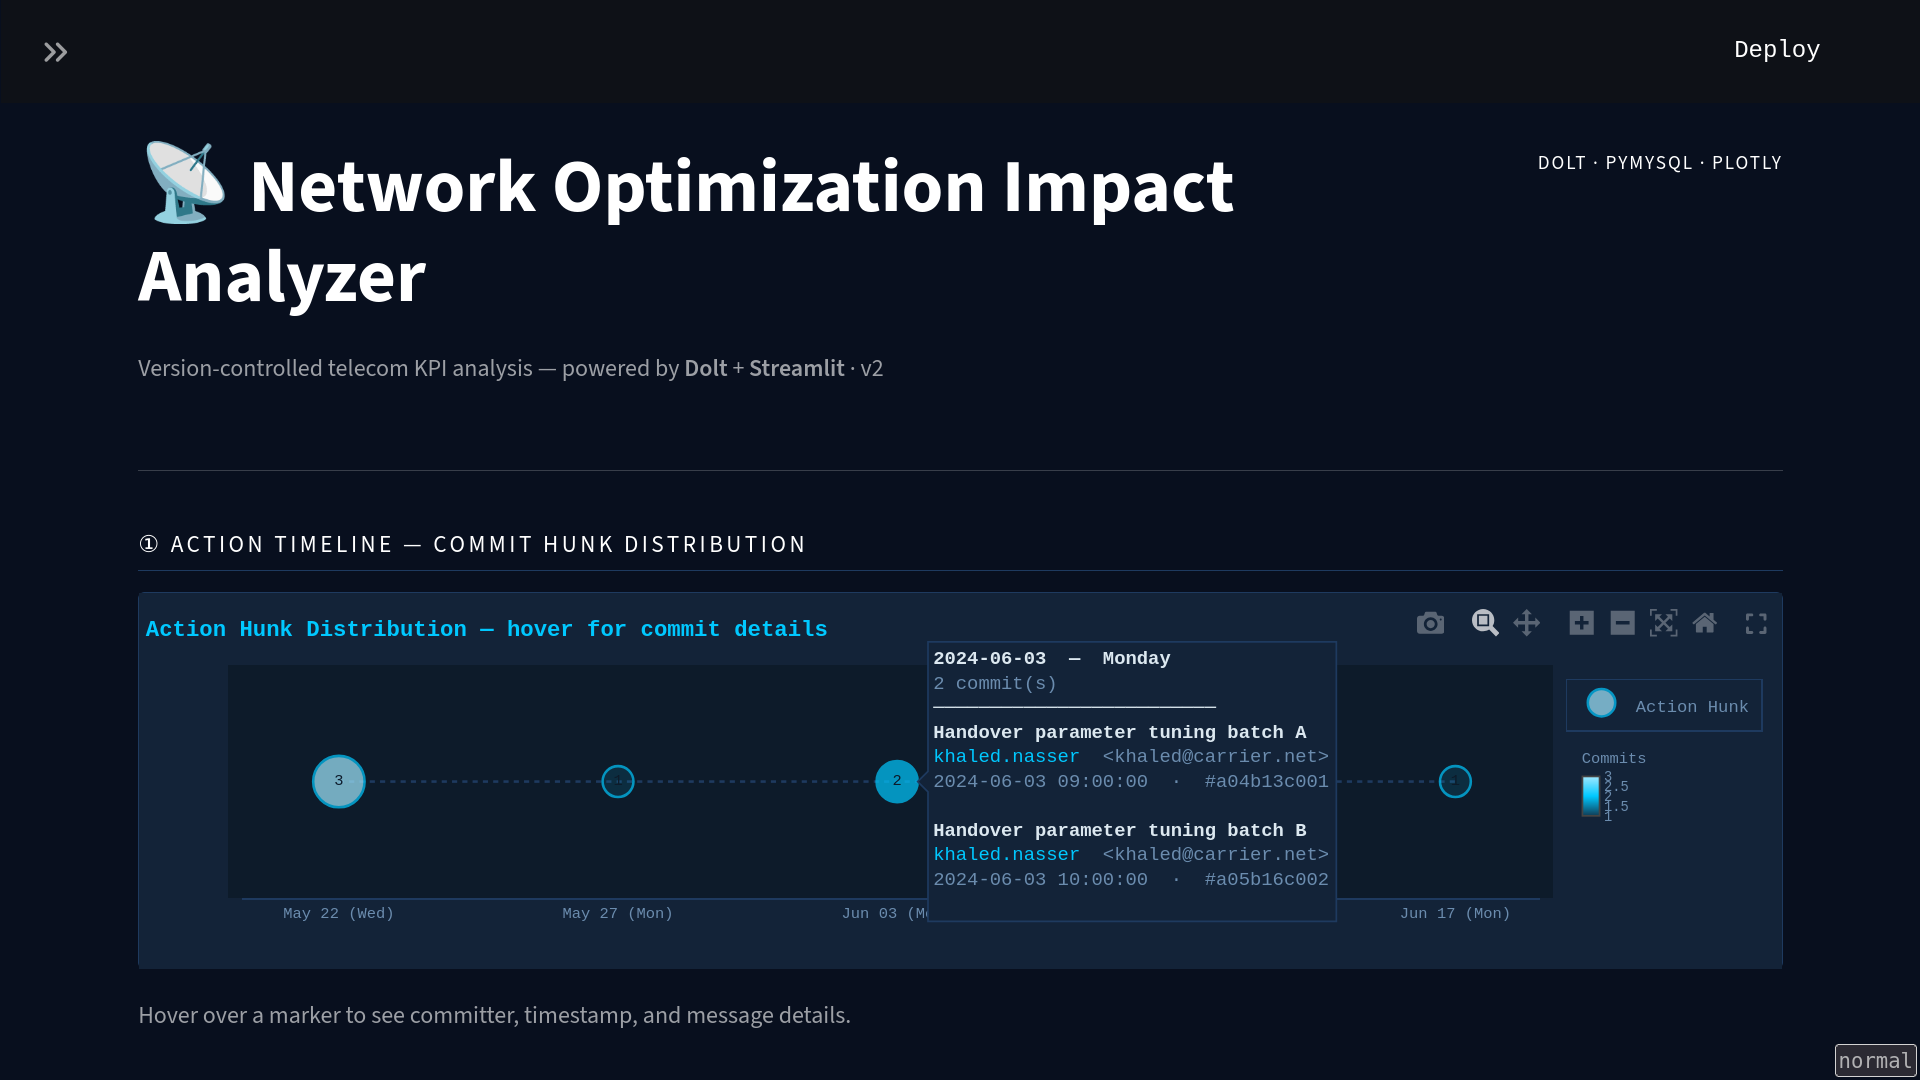
\includegraphics[width=0.85\textwidth]{figures/chapter06/action_timeline.png}
    \caption{Action Timeline HUD showing five Action Hunks with
    per-commit hover detail. \emph{[Screenshot placeholder]}}
    \label{fig:screenshot-timeline}
\end{figure}

\begin{figure}[htbp]
    \centering
    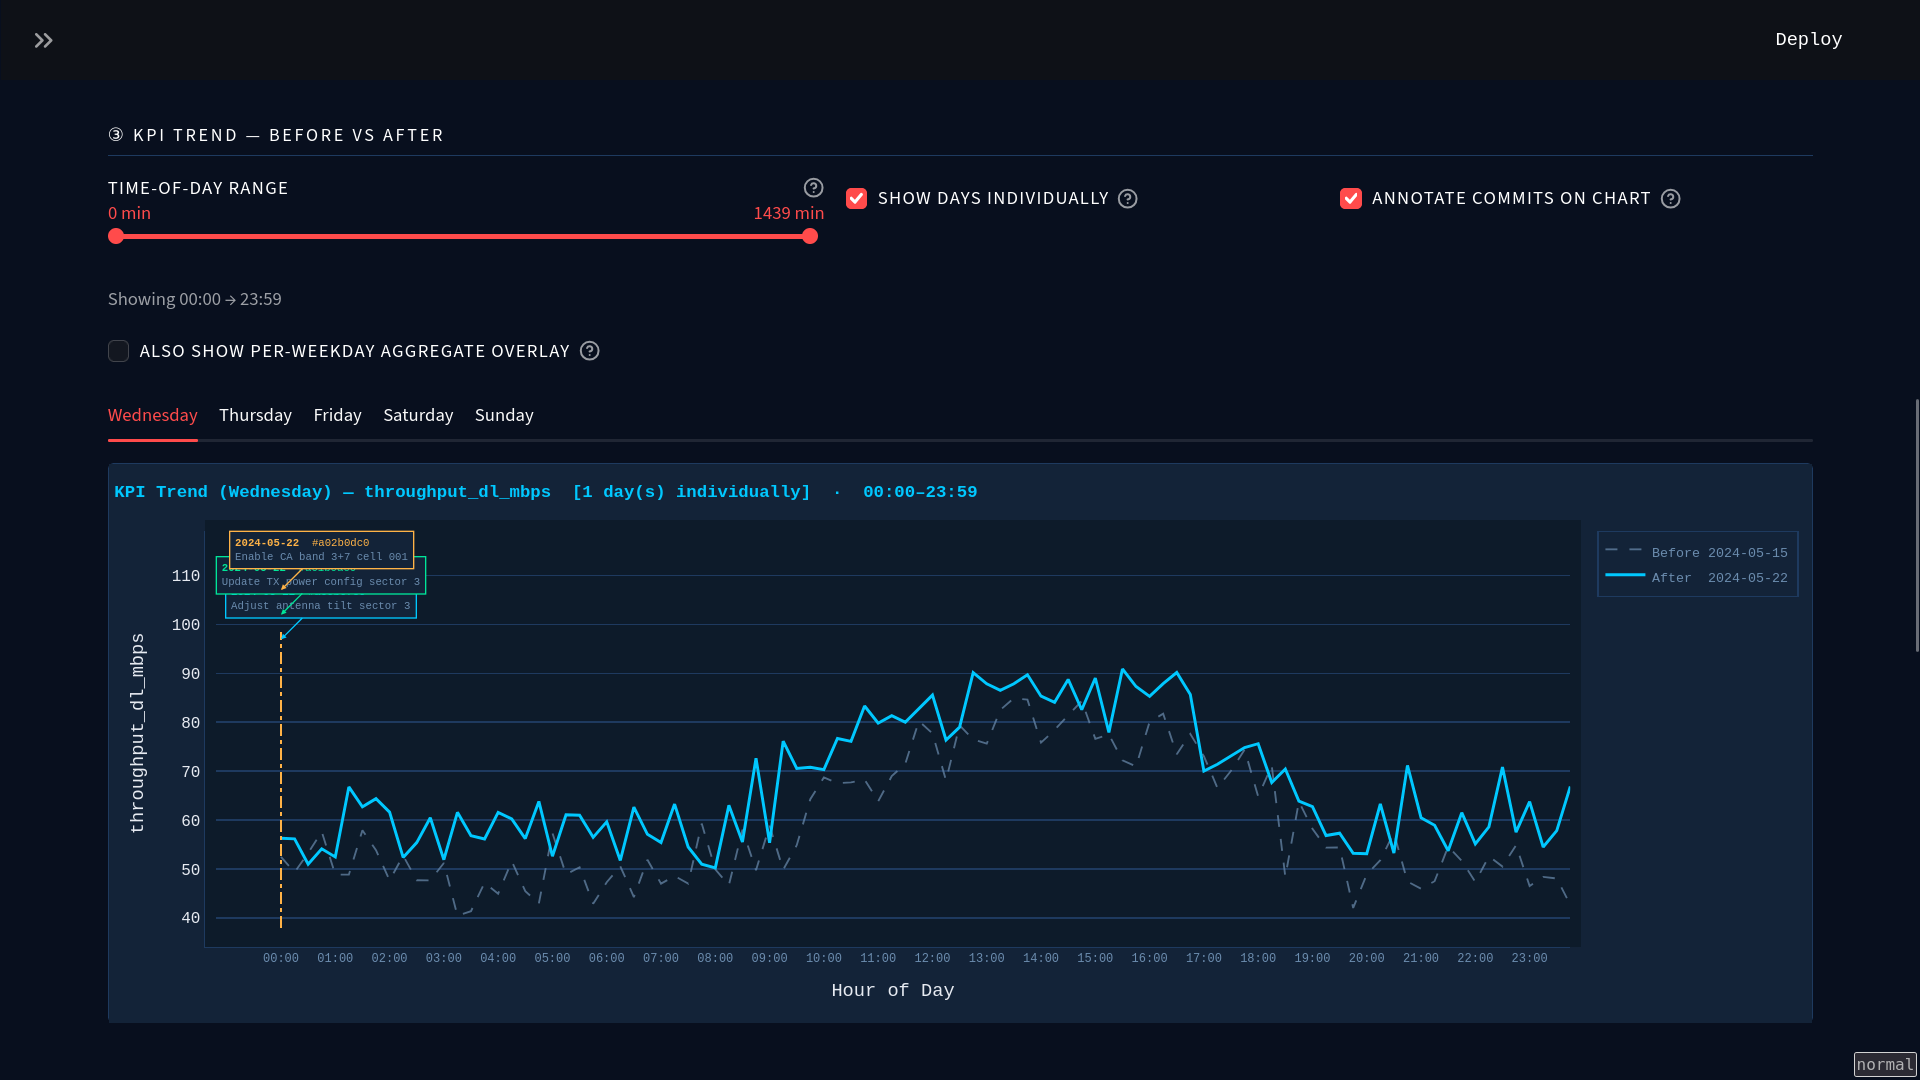
\includegraphics[width=0.85\textwidth]{figures/chapter06/kpi_trend.png}
    \caption{Before/After KPI trend comparison for a selected metric,
    with commit annotations. \emph{[Screenshot placeholder]}}
    \label{fig:screenshot-trend}
\end{figure}

\begin{figure}[htbp]
    \centering
    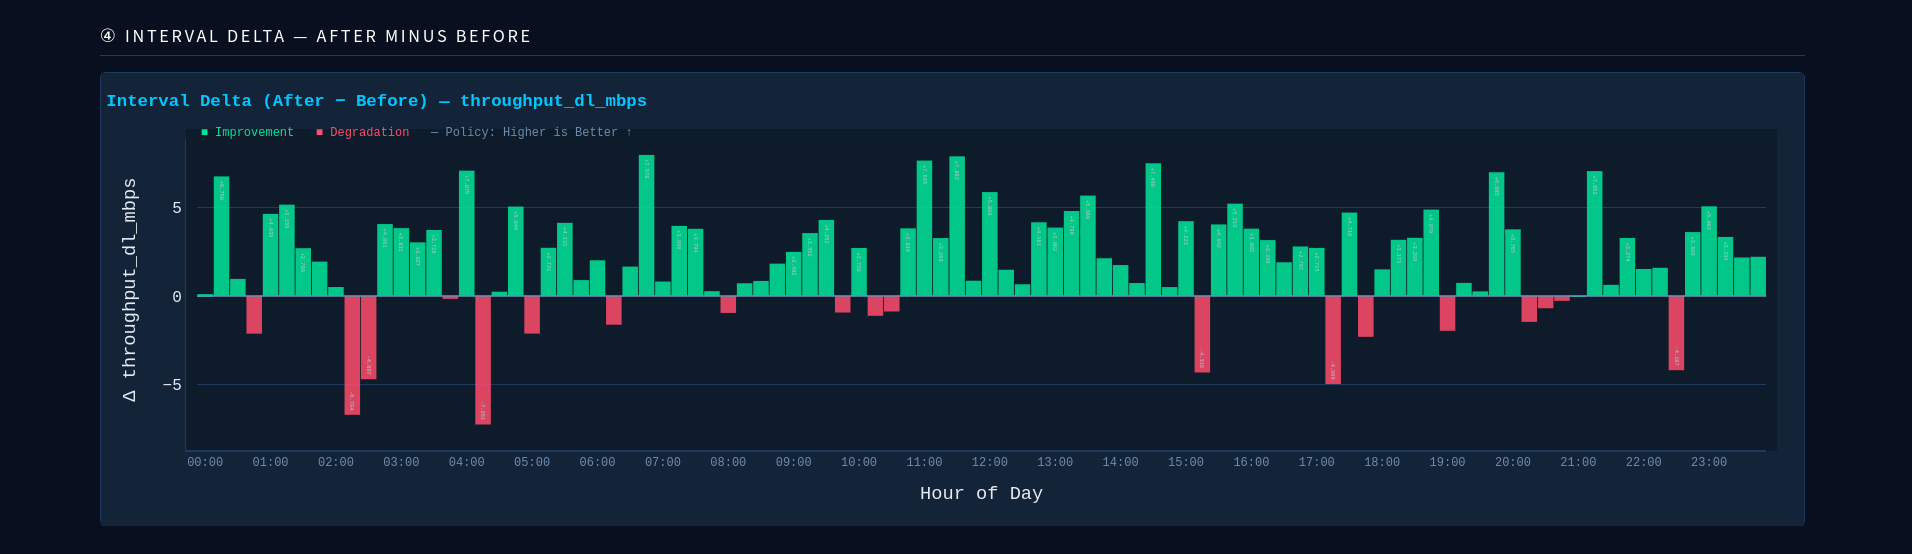
\includegraphics[width=0.85\textwidth]{figures/chapter06/delta_bars.png}
    \caption{Polarity-aware interval delta bar chart. \emph{[Screenshot
    placeholder]}}
    \label{fig:screenshot-delta}
\end{figure}

\begin{figure}[htbp]
    \centering
    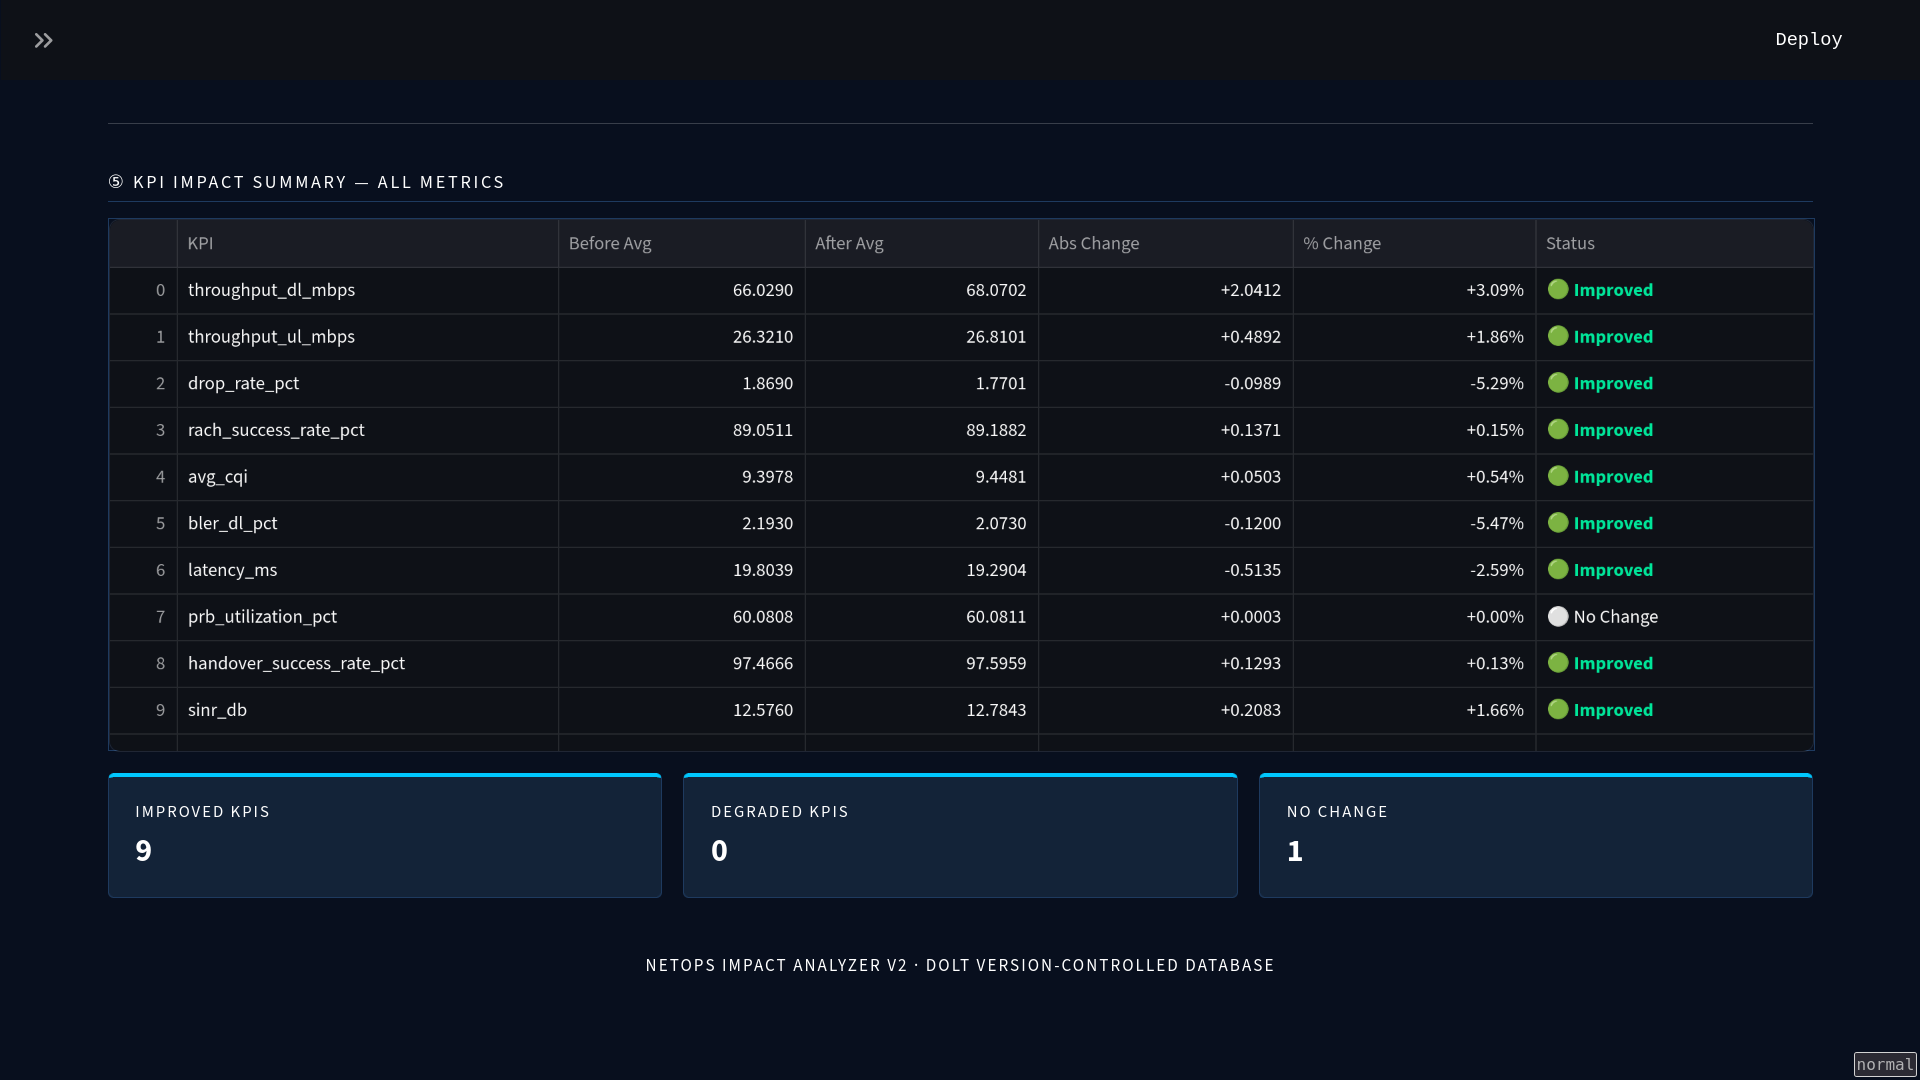
\includegraphics[width=0.85\textwidth]{figures/chapter06/summary_table.png}
    \caption{KPI impact summary table with Improved/Degraded/No-Change
    status counts. \emph{[Screenshot placeholder]}}
    \label{fig:screenshot-summary}
\end{figure}

\section{User Workflow}
The Streamlit application (\texttt{app.py}) guides the analyst through a
linear, five-section workflow, illustrated in
Figure~\ref{fig:workflow} and summarised below.

\begin{figure}[htbp]
    \centering
    \begin{tikzpicture}[
        node distance=6mm,
        stepbox/.style={draw, rounded corners, fill=cyan!8,
                     minimum width=9.5cm, minimum height=0.9cm,
                     align=left, font=\small},
        arrow/.style={-{Latex[length=2mm]}, thick}
    ]
        \node[stepbox] (s1) {\textbf{\textcircled{1}} Action Timeline --- browse all Action Hunks};
        \node[stepbox, below=of s1] (s2) {\textbf{\textcircled{2}} Select Action Hunk + KPI + evaluation window options};
        \node[stepbox, below=of s2] (s3) {\textbf{\textcircled{3}} KPI Trend --- Before vs. After (aggregated or per-day)};
        \node[stepbox, below=of s3] (s4) {\textbf{\textcircled{4}} Interval Delta --- After minus Before, polarity-coded};
        \node[stepbox, below=of s4] (s5) {\textbf{\textcircled{5}} KPI Impact Summary --- all metrics, one table};
        \draw[arrow] (s1) -- (s2);
        \draw[arrow] (s2) -- (s3);
        \draw[arrow] (s3) -- (s4);
        \draw[arrow] (s4) -- (s5);
    \end{tikzpicture}
    \caption{The five-step analyst workflow implemented in \texttt{app.py}.}
    \label{fig:workflow}
\end{figure}

\begin{enumerate}
    \item \textbf{Action Timeline.} The analyst first sees every Action
        Hunk plotted on an interactive timeline, giving immediate visual
        context on how frequently and when optimization actions have
        occurred.
    \item \textbf{Hunk \& Window Selection.} The analyst picks a specific
        hunk, a KPI to analyse, and optionally toggles \emph{Ignore Next
        Action Hunk} to extend the evaluation window past a later
        change. Metric tiles immediately display the resolved Action
        Date, After-window end date, next-hunk boundary (if any), and
        matched weekday. An expandable panel additionally surfaces the
        exact configuration diff (table, column, from-value, to-value)
        for every commit in the hunk, sourced live from Dolt's
        \texttt{dolt\_diff\_*} system views.
    \item \textbf{KPI Trend.} The Before/After profiles are rendered
        either as a single aggregated pair of curves or, when multiple
        After days exist, split per weekday with each individual day
        plotted against its matched baseline. A time-of-day slider lets
        the analyst zoom into a specific part of the day (e.g. business
        hours only).
    \item \textbf{Interval Delta.} A bar chart quantifies the exact
        magnitude and direction of change at every time-of-day interval,
        automatically colour-coded using the KPI's configured polarity.
    \item \textbf{Impact Summary.} A single sortable table reports
        Before/After averages, absolute and percentage change, and an
        Improved/Degraded/No-Change verdict for \emph{every} KPI in the
        dataset simultaneously, with roll-up counts displayed as summary
        tiles.
\end{enumerate}

\section{Technology Stack}
\begin{table}[htbp]
    \centering
    \caption{Technologies used in the Optimization Action Analyzer}
    \label{tab:stack}
    \begin{tabular}{@{}ll@{}}
        \toprule
        \textbf{Layer} & \textbf{Technology} \\
        \midrule
        Database              & Dolt (version-controlled MySQL-compatible SQL server) \\
        Database connector    & PyMySQL \\
        Data processing        & pandas, NumPy \\
        Visualization          & Plotly (\texttt{plotly.graph\_objects}) \\
        Web application / UI   & Streamlit \\
        Configuration persistence & JSON (\texttt{kpi\_config.json}) \\
        \bottomrule
    \end{tabular}
\end{table}

\section{Design Highlights}
\begin{itemize}
    \item \textbf{Version control as the audit trail.} By building on
        Dolt rather than a conventional relational database, every
        configuration change is inherently versioned, attributable, and
        diffable --- eliminating the need for a bespoke change-log
        table.
    \item \textbf{Seasonality-aware statistics.} The weekday-matching
        baseline logic (Section~\ref{chap:opt-action-analyzer}, Core
        Algorithms) avoids the common pitfall of comparing traffic across
        mismatched days of the week.
    \item \textbf{Automatic boundary detection.} The rolling evaluation
        window automatically caps itself at the next recorded change,
        preventing the effects of two overlapping optimization actions
        from being conflated, while still giving the analyst an explicit
        override.
    \item \textbf{Zero-configuration KPI discovery.} New KPI columns
        added to the \texttt{network\_kpis} table are automatically
        discovered via \texttt{INFORMATION\_SCHEMA} introspection and
        assigned a sensible default polarity, requiring no code changes
        to support new metrics.
    \item \textbf{Graceful degradation.} A mock-data mode
        (\texttt{USE\_MOCK\_DATA}) allows the entire application --- UI,
        charts, and analysis logic --- to be demonstrated and developed
        without a live Dolt deployment.
\end{itemize}

\section{Limitations and Future Work}
\begin{itemize}
    \item The current workflow depends on the dolt version-control system which is yet to be adopted in the workflow of the filed optimization.
    \item Statistical significance testing (e.g. confidence intervals or
        hypothesis tests on the Before/After delta) is not yet
        implemented; the summary table currently reports point
        estimates only.
    \item The tool currently analyses one cell/site's KPI stream at a
        time; extending the schema and queries to support multi-cell,
        multi-site comparative analysis is a natural next step.
    \item Anomaly detection could be layered on top of the delta bar
        chart to automatically flag intervals with statistically
        unusual deviations, rather than relying solely on the polarity
        sign convention.
\end{itemize}

\section{Summary}
The Optimization Action Analyzer demonstrates how pairing a
version-controlled database with a seasonality-aware statistical
comparison engine and an interactive visualization layer can turn a
traditionally manual, error-prone impact-assessment workflow into a
repeatable, auditable, and self-service analytical tool. By automatically
reconstructing the timeline of network changes from the database's own
commit history and comparing performance against weekday-matched
baselines, the system gives network optimization teams a fast, reliable
answer to the central question of their work: \emph{did this change
actually help?}
